\subsection{2D Transient Conduction - 4 Materials Case}~\label{secDiffusion2D}
In this section, the implementation of a heat conduction model for the \textbf{4 Materials Case} will be developed. The problem consists of the rectangular domain shown in Fig.~\ref{fig4Materials}, which is composed by 4 different materials with their thermophysical properties being listed in Table~\ref{tab2DMaterials}. Furthermore, the domain has an initial value of $T_0 = 8 ^\circ C$ and is bound by the boundary conditions shown in Table~\ref{tab4MaterialBC}.

\begin{figure}[ht]
    \centering
    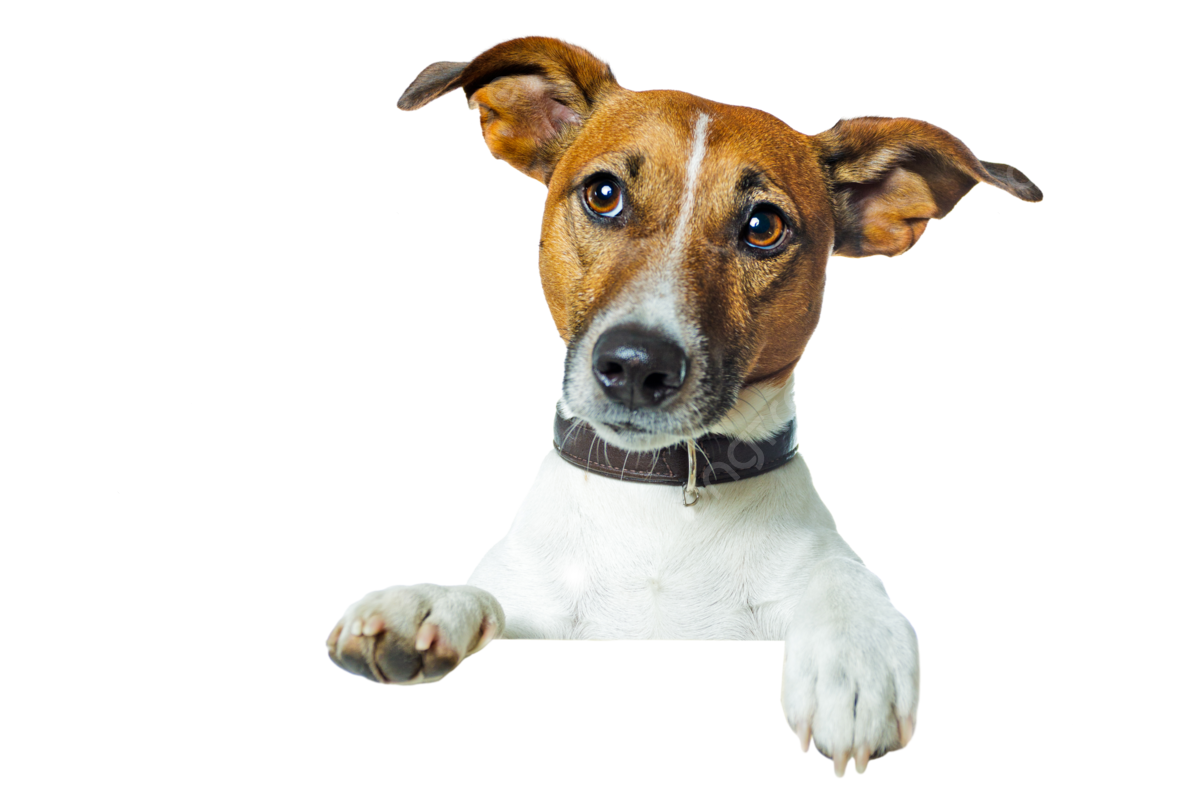
\includegraphics[width=0.45\linewidth]{Chapter1/Media/PLACEHOLDER.png}
    \caption{Diagram for 4 Materials Case.}
    \label{fig4Materials}
\end{figure}

\begin{table}[ht]
    \centering
    \begin{tabular}{|c|c|c|c|}
        \hline
        \multirow{2}{*}{Material} & $\rho$ & $c_P$ & $\lambda$ \\
                                  & $[kg/m^3]$ & $[J/(kg \cdot K)]$ & $[W/(mK)]$ \\
        \hline
        M1 & 1500 & 750 & 160 \\ 
        M2 & 1600 & 770 & 140 \\
        M3 & 1900 & 810 & 200 \\
        M4 & 2500 & 930 & 140 \\
        \hline
    \end{tabular}
    \caption{Thermophysical properties of the four materials in the domain.}
    \label{tab2DMaterials}
\end{table}

\begin{table}[ht]
    \centering
    \begin{tabular}{|c|l|}
        \hline
        Cavity Wall & Boundary Condition \\
        \hline
        West & \textbf{Robin}: In contact with fluid at $T_f = 33 ^\circ C$ and $h = 9 \, W/(m^2 K)$ \\
        East & \textbf{Dirichlet}: Uniform temperature $T(t) = 8 + 0.005 t ^\circ C$ \\
        South & \textbf{Dirichlet}: Uniform temperature $T = 23 ^\circ C$ \\
        North & \textbf{Neumann}: Uniform $\dot{Q}_{flow}$ \\
        \hline
    \end{tabular}
    \caption{Boundary conditions for the 4 Materials Case domain.}
    \label{tab4MaterialBC}
\end{table}


\subsubsection{Model Implementation}
The model developed for the 2D case will follow the same discretization proposed earlier for the 1D case. However, some modifications to the code structure were needed to support the new functionalities. For example, Probe was expanded to support different types of probes with a better control over the region of the domain that is desired. A summary of the modified parameters included in this iteration of the model is shown in Table~\ref{tabConfig2D}, summarizing the new parameters in the configuration file. As shown, Probes have now been added as a configurable parameter to allow the user to choose which data is being saved. In addition, refinement was modified to be defined independently for each axis and in separate regions to allow the user better control over the mesh. Furthermore, a Medic class was also included to handle diagnostics and validation of energy conservation in the system. This class is also used as the central tool for debugging as it can easily be modified to log any information relevant to the model.

\begin{table}[ht]
	\centering
	\begin{tabular}{|l|c|p{0.5\linewidth}|}
		\hline
		Group & Parameter & Description \\
		\hline
        \multirow{4}{*}{Mesh Data} & \multirow{2}{*}{N} & List specifying total number of nodes for each axis. \\
					   & \multirow{2}{*}{refinement} & List of vectors specifying refinement configuration for each axis. \\
		\hline
		\multirow{2}{*}{Probe Data} & \multirow{2}{*}{probes} & List of vectors specifying the probes configured for the simulation. \\
		\hline
	\end{tabular}
	\caption{Configuration file structure changes, highlighting the expansion in mesh refinement capacity and probe flexibility.}
	\label{tabConfig2D}
\end{table}

\subsubsection{Numerical Parameter Study}
For this test, timestep $\Delta t$ and number of nodes $N$ are modified to analyze their impact on the number of iterations and total residue. Both parameters will be independently swept across their respective range of values while keeping the other parameter at a constant value. A summary of the values for each of these parameters is shown in Table \ref{tabDiffNumerical2D}, highlighting the values used for the base case. In addition, the explicit scheme still requires an imposed limit for the value of $\Delta t$; however the expression for the 2D case changes as described by Eq. \ref{eqDiffExplicit2D} due to the presence of simultaneous diffusion in both axis. Contrary to the results shown for the 1D case, there will be no comparison of error with the analytical solution or computation time. This numerical parameter study will focus on comparing the number of iterations and total residue.

\begin{table}[ht]
	\centering
	\begin{tabular}{|c|c|}
		\hline
		Parameter & Values \\
		\hline
		$\Delta t$ & 0.1, 0.5, \textbf{1.0}, 2.0, 5.0 \\
		$N$ & 50, \textbf{100}, 200, 400 \\
		\hline
	\end{tabular}
	\caption{Value ranges for numerical parameter study.}
	\label{tabDiffNumerical2D}
\end{table}

\begin{equation}
	\label{eqDiffExplicit2D}
\Delta t_{max} = \frac{\Delta x^2 \Delta y^2}{2 \alpha (\Delta x^2 + \Delta y^2)}
\end{equation}

\paragraph{$\Delta t$ Study}
The results obtained from the tests explained above are shown in Figure \ref{figDiffResults2DA}. As shown, the number of iterations and total residue follow a similar trend to the one seen in the 1D case, increasing with $\Delta t$ for the implicit and Crank-Nicolson schemes, showing a better performance for the Crank-Nicolson scheme on both metrics.  On the other hand, the explicit scheme did not present any changes during the timestep study. This is due to the timestep being limited by the expression discussed above; which activated for all analyzed cases.

\begin{figure}[ht]
	\begin{tabular}{cc}
		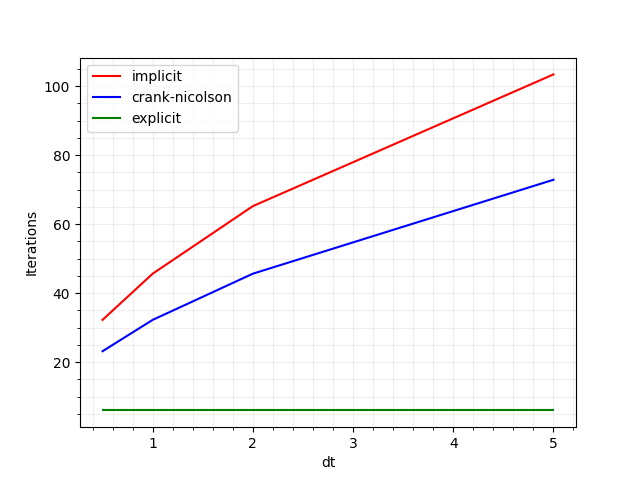
\includegraphics[width=0.45\linewidth]{Chapter1/Media/tSweep2DIterations.png} & 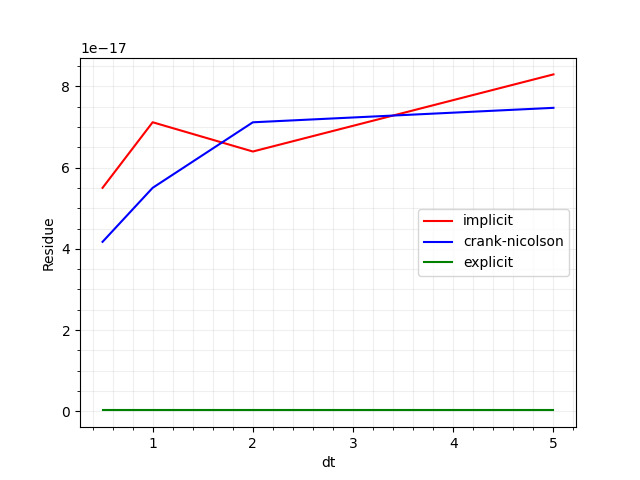
\includegraphics[width=0.45\linewidth]{Chapter1/Media/tSweep2DResidue.png} \\
	\end{tabular}
	\caption{$\Delta t$ sweep results.}
	\label{figDiffResults2DA}
\end{figure}

\paragraph{$N$ Study}
The results obtained from the tests explained above are shown in Figure \ref{figDiffResults2DB}. Just like in the previous test, the presented plots show a similar trend to the one seen in the previous scenario, showing an increase in number of iterations and residue for most cases. Furthermore, the implicit scheme showed higher sensitivity to increases in $N$ compared to the Crank-Nicolson and explicit schemes; with the explicit scheme showing no change at all. On the other hand, while residue was significantly higher for implicit on coarser meshes, the difference between the implicit and Crank-Nicolson schemes became smaller as $N$ increased; with the explicit scheme showing a slight increase in the beginning but less of an impact as $N$ kept increasing.

\begin{figure}[ht]
    \centering
	\begin{tabular}{cc}
		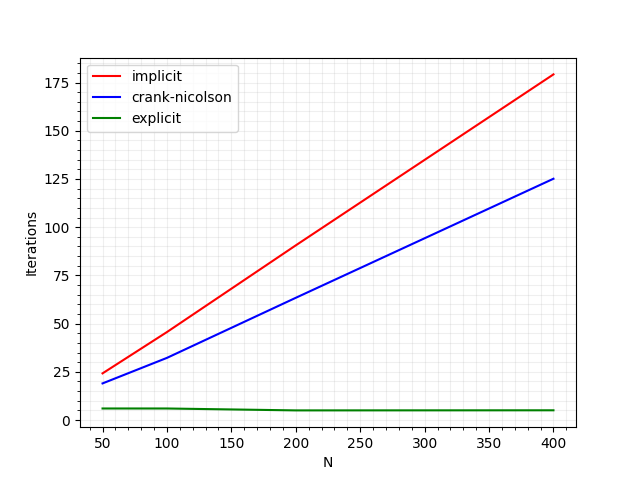
\includegraphics[width=0.45\linewidth]{Chapter1/Media/NSweep2DIterations.png} & 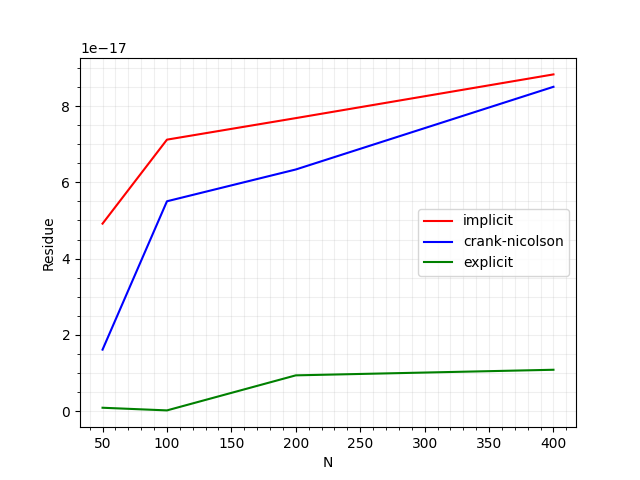
\includegraphics[width=0.45\linewidth]{Chapter1/Media/NSweep2DResidue.png} \\
	\end{tabular}
	\caption{$N$ sweep results.}
	\label{figDiffResults2DB}
\end{figure}

\subsubsection{Model Validation}
As a preliminary step, the three boundary condition types (Dirichlet, Neumann, and Robin) were independently verified in 2D by applying an adiabatic Neumann condition ($\partial T / \partial n = 0$) on the faces of the secondary axis, effectively reducing the problem to a 1D configuration along the primary axis. The results successfully replicated the steady-state profiles validated in Section~\ref{secDiffusion1D} for each axis, confirming that the boundary condition implementation is correct in two dimensions.

The primary benchmark for this chapter is the \textbf{4 Materials Case}~\cite{}, whose results are shown in Fig.~\ref{figDiff2D4Materials}. Since this is a transient simulation, no closed-form analytical solution exists; validation is instead performed against reference temperatures at two probe locations, $[0.65, 0.56]$ and $[0.74, 0.72]$, at prescribed time instants. The model successfully matched both reference values and produced a temperature distribution consistent with the expected evolution of the domain.

\begin{figure}[ht]
	\centering
	\begin{tabular}{cc}
		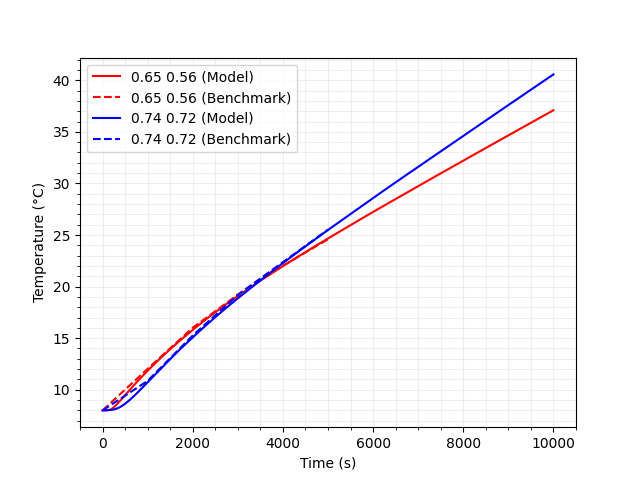
\includegraphics[width=0.45\linewidth]{Chapter1/Media/4MaterialsPoint.png} & 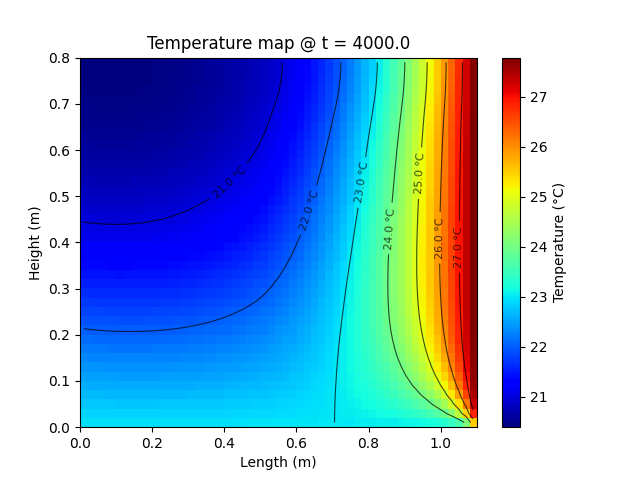
\includegraphics[width=0.45\linewidth]{Chapter1/Media/4MaterialsMap.png} \\
	\end{tabular}
	\caption{Comparison of probe temperatures against reference values (left) and steady-state temperature distribution (right) for the 4 Materials Case.}
	\label{figDiff2D4Materials}
\end{figure}

